\chapter{Resultados preliminares}
\label{chap:resultados-preliminares}
Neste capítulo, apresentaremos os resultados preliminares obtidos através de uma análise descritiva. Os resultados estão segmentados por gênero e situação de aprovação nos cursos inscritos.

\section{Perfil dos candidatos, instituições de ensino e cursos de graduação}
Para descrever o perfil dos participantes e cursos de graduação, realizamos um levantamento através de algumas variáveis específicas. No conjunto de dados do ENEM, a análise foi segmentada por gênero, observado na \autoref{tab:estatistica-enem}. As mulheres constituem 58\% do total de candidatos, ao passo que homens constituem 32\%. Escolas públicas de nível estadual concentram a maioria dos estudantes. Em relação à escolaridade, a maior parte das mães possui ensino médio completo, enquanto a maioria dos pais não possui ensino médio completo. A faixa etária com mais estudantes é de 16 a 20 anos, sendo que a idade que possui mais candidatos é a de 17 anos. Quanto à identificação racial, brancos e pardos concentram a maioria do total. Já no SISU, a segmentação é realizada por situação de aprovação, observada na \autoref{tab:estatistica-sisu}. Aprovados são 4,4,4\% do total e reprovados 95,6\%. Cursos de grau bacharelado e licenciatura e de turno integral e noturno são os que possuem mais inscrições. Observamos que homens possuem mais aprovações, ao passo que mulheres são a maioria dos não aprovados. Ações afirmativas beneficiam mais da metade dos participantes, em ambos os segmentos.

\begin{table}[h]
    \begin{tabular}{cccc}
    \hline
    \textbf{}                                   & \textbf{Gênero}           & Feminino & Masculino \\ \hline
    \textbf{Variável}                           & \textbf{Descrição}        & \textbf{}         & \textbf{}          \\ \hline
    \multirow{4}{*}{\begin{tabular}[c]{@{}c@{}}Dependência\\administrativa\\da escola\end{tabular}} & Estadual                  & 77,33\%           & 73,80\%            \\ \cline{2-4} 
                                                & Federal                   & 2,21\%            & 2,99\%             \\ \cline{2-4} 
                                                & Municipal                 & 0,92\%            & 0,88\%             \\ \cline{2-4} 
                                                & Privada                   & 19,53\%           & 22,32\%            \\ \hline
    \multirow{2}{*}{Escolaridade mãe}           & Com EM completo & 50,26\%           & 55,69\%            \\ \cline{2-4} 
                                                & Sem EM completo & 49,74\%           & 44,31\%            \\ \hline
    \multirow{2}{*}{Escolaridade pai}           & Com EM completo & 39,01\%           & 44,72\%            \\ \cline{2-4} 
                                                & Sem EM completo & 60,99\%           & 55,28\%            \\ \hline
    \multirow{9}{*}{Idade}                      & 15 anos ou menos          & 0,16\%            & 0,11\%             \\ \cline{2-4} 
                                                & 16 a 20 anos              & 97,15\%           & 96,97\%            \\ \cline{2-4} 
                                                & 21 a 25 anos              & 1,78\%            & 2,38\%             \\ \cline{2-4} 
                                                & 26 a 30 anos              & 0,39\%            & 0,28\%             \\ \cline{2-4} 
                                                & 31 a 35 anos              & 0,23\%            & 0,11\%             \\ \cline{2-4} 
                                                & 36 a 40 anos              & 0,14\%            & 0,06\%             \\ \cline{2-4} 
                                                & 41 a 45 anos              & 0,08\%            & 0,04\%             \\ \cline{2-4} 
                                                & 46 a 50 anos              & 0,04\%            & 0,02\%             \\ \cline{2-4} 
                                                & 50 anos ou mais           & 0,03\%            & 0,02\%             \\ \hline
    \multirow{7}{*}{Raça}                       & Amarela                   & 2,45\%            & 1,86\%             \\ \cline{2-4} 
                                                & Branca                    & 40,53\%           & 41,57\%            \\ \cline{2-4} 
                                                & Indígena                  & 0,54\%            & 0,61\%             \\ \cline{2-4} 
                                                & Não declarado             & 1,44\%            & 1,83\%             \\ \cline{2-4} 
                                                & Parda                     & 44,30\%           & 42,40\%            \\ \cline{2-4} 
                                                & Preta                     & 10,73\%           & 11,72\%            \\ \cline{2-4} 
                                                & Sem informação            & 0,00\%            & 0,00\%             \\ \hline
    \end{tabular}
    \caption{Estatísticas descritivas dos participantes do ENEM por gênero}
    \label{tab:estatistica-enem}
    \end{table}

\begin{table}[h]
    \centering
    \begin{tabular}{cccc}
    \hline
    \textbf{}                   & \textbf{Situação}             & Aprovado  & Não aprovado \\ \hline
    \textbf{Variável}           & \textbf{Descrição}            & \textbf{} & \textbf{}    \\ \hline
    \multirow{4}{*}{Grau}       & Bacharelado                   & 62,82\%   & 66,39\%      \\ \cline{2-4} 
                                & Licenciatura                  & 26,08\%   & 21,62\%      \\ \cline{2-4} 
                                & Tecnológico                   & 7,48\%    & 9,52\%       \\ \cline{2-4} 
                                & Área Básica de Ingresso (ABI) & 3,63\%    & 2,46\%       \\ \hline
    \multirow{2}{*}{Gênero}     & Feminino                      & 46,49\%   & 57,94\%      \\ \cline{2-4} 
                                & Masculino                     & 53,51\%   & 42,06\%      \\ \hline
    \multirow{2}{*}{Modalidade} & Ampla concorrência            & 45,78\%   & 45,76\%      \\ \cline{2-4} 
                                & Ações afirmativas             & 54,22\%   & 54,24\%      \\ \hline
    \multirow{4}{*}{Turno}      & Integral                      & 44,27\%   & 45,34\%      \\ \cline{2-4} 
                                & Matutino                      & 12,34\%   & 12,28\%      \\ \cline{2-4} 
                                & Noturno                       & 35,45\%   & 34,67\%      \\ \cline{2-4} 
                                & Vespertino                    & 7,94\%    & 7,70\%       \\ \hline
    \end{tabular}
    \caption{Estatísticas descritivas de cursos e participantes do SISU por situação de aprovação}
    \label{tab:estatistica-sisu}
    \end{table}

Também é levantado o desempenho dos estudantes nas provas do exame. No ENEM, em todas as provas, para ambos os gêneros, o intervalo de notas que possui a maior observação é o de (400, 600]. A observação das notas em intervalos pode ser vista na \autoref{tab:observacao-nota-enem}, e sua distribuição em gráfico de densidade na \autoref{fig:nota-genero}, divididas por gênero. No SISU, aprovados tendem a se concentrar em intervalos com maiores notas, como (600, 800] e (800, 1000] na redação, enquanto não aprovados se concentram em (400, 600]. De forma similar, isso pode ser visto na \autoref{tab:observacao-nota-sisu} e na \autoref{fig:nota-aprovacao}, divididas por situação de aprovação. As estatística descritivas, com cálculo de média, desvio padrão e p-valor resultante da aplicação de teste t, estão disponíveis para o ENEM na \autoref{tab:estatistica-nota-enem} e para o SISU na \autoref{tab:estatistica-nota-sisu}. Homens possuem maiores médias de notas objetivas e mulheres possuem maior média de nota em redação. Aprovados possuem maiores médias em todas as provas. Em ambos os conjuntos, temos os resultados do p-valor zerados, mostrando que a diferença nas médias é estatisticamente significativa.

A \autoref{tab:classificacao-curso-genero} mostra a classificação das áreas dos cursos por gênero. As áreas mais ocupadas por mulheres são Saúde e bem-estar e Ciências sociais, negócios e direito, enquanto as áreas mais ocupadas por homens são Ciência e Ciências sociais, negócios e direito. Com relação à proporção de homens e mulheres por área, homens são maioria nas áreas de Ciência (55,4\%) e Engenharia, manufatura e construção (60,25\%). A \autoref{tab:universidade-inscricao} mostra a distribuição das universidades com mais inscrições. As 3 instituições com mais inscritos são as universidades federais do Maranhão, Rio de Janeiro e Fluminense. A \autoref{fig:distribuicao-uf} mostra a distribuicao das unidades federativas no SISU, divididas pelas inscrições em instituições de ensino e residência dos candidatos. As IES com mais inscrições localizam-se nos estados de Minas Gerais, Rio de Janeiro e Bahia, ao passo que os estados de residência com mais candidatos são Minas Gerais, São Paulo e Rio de Janeiro. 
   
\begin{table}[h]
    \centering
    \begin{tabular}{ccccccc}
    \hline
    \multicolumn{2}{c}{\textbf{Intervalo}}                                                                & \multicolumn{1}{l}{(0, 200{]}} & (200, 400{]} & (400, 600{]} & (600, 800{]} & (800, 1000{]} \\ \hline
    \textbf{Prova}                                                                            & \textbf{Gênero}    &                                &              &              &              &               \\ \hline
    \multirow{2}{*}{\begin{tabular}[c]{@{}c@{}}Ciências\\ Humanas\end{tabular}}      & Feminino  & 0,00\%                         & 4,06\%       & 78,43\%      & 17,51\%      & 0,01\%        \\ \cline{2-7} 
                                                                                     & Masculino & 0,00\%                         & 3,90\%       & 71,81\%      & 24,28\%      & 0,02\%        \\ \hline
    \multirow{2}{*}{\begin{tabular}[c]{@{}c@{}}Ciências da \\ Natureza\end{tabular}} & Feminino  & 0,00\%                         & 12,75\%      & 80,99\%      & 6,25\%       & 0,00\%        \\ \cline{2-7} 
                                                                                     & Masculino & 0,00\%                         & 9,14\%       & 80,03\%      & 10,80\%      & 0,03\%        \\ \hline
    \multirow{2}{*}{Linguagens}                                                      & Feminino  & 0,00\%                         & 4,18\%       & 83,41\%      & 12,42\%      & 0,00\%        \\ \cline{2-7} 
                                                                                     & Masculino & 0,00\%                         & 4,51\%       & 81,05\%      & 14,44\%      & 0,00\%        \\ \hline
    \multirow{2}{*}{Matemática}                                                      & Feminino  & 0,00\%                         & 22,11\%      & 66,32\%      & 11,02\%      & 0,55\%        \\ \cline{2-7} 
                                                                                     & Masculino & 0,00\%                         & 13,67\%      & 63,26\%      & 21,16\%      & 1,90\%        \\ \hline
    \multirow{2}{*}{Redação}                                                         & Feminino  & 0,24\%                         & 11,00\%      & 57,36\%      & 26,08\%      & 5,32\%        \\ \cline{2-7} 
                                                                                     & Masculino & 0,43\%                         & 15,48\%      & 58,48\%      & 21,72\%      & 3,88\%        \\ \hline
    \end{tabular}
    \caption{Observações de notas dos participantes do ENEM por gênero}
    \label{tab:observacao-nota-enem}
    \end{table}

\begin{table}[h]
\centering
\begin{tabular}{ccccccc}
\hline
\multicolumn{2}{c}{\textbf{Intervalo}}                                                                   & \multicolumn{1}{l}{(0, 200{]}} & (200, 400{]} & (400, 600{]} & (600, 800{]} & (800, 1000{]} \\ \hline
\textbf{Prova}                                                                            & \textbf{Situação}     &                                &              &              &              &               \\ \hline
\multirow{2}{*}{\begin{tabular}[c]{@{}c@{}}Ciências\\ Humanas\end{tabular}}      & Aprovado     & 0,00\%                         & 0,02\%       & 20,60\%      & 79,19\%      & 0,18\%        \\ \cline{2-7} 
                                                                                 & Não aprovado & 0,06\%                         & 1,95\%       & 69,81\%      & 28,16\%      & 0,02\%        \\ \hline
\multirow{2}{*}{\begin{tabular}[c]{@{}c@{}}Ciências da \\ Natureza\end{tabular}} & Aprovado     & 0,00\%                         & 0,30\%       & 53,09\%      & 46,42\%      & 0,19\%        \\ \cline{2-7} 
                                                                                 & Não aprovado & 0,06\%                         & 7,80\%       & 80,93\%      & 11,19\%      & 0,02\%        \\ \hline
\multirow{2}{*}{Linguagens}                                                      & Aprovado     & 0,00\%                         & 0,15\%       & 42,26\%      & 57,59\%      & 0,00\%        \\ \cline{2-7} 
                                                                                 & Não aprovado & 0,01\%                         & 2,44\%       & 79,82\%      & 17,73\%      & 0,00\%        \\ \hline
\multirow{2}{*}{Matemática}                                                      & Aprovado     & 0,00\%                         & 1,47\%       & 32,22\%      & 57,44\%      & 8,87\%        \\ \cline{2-7} 
                                                                                 & Não aprovado & 0,01\%                         & 14,04\%      & 64,61\%      & 19,88\%      & 1,46\%        \\ \hline
\multirow{2}{*}{Redação}                                                         & Aprovado     & 0,24\%                         & 0,22\%       & 15,26\%      & 53,90\%      & 30,62\%       \\ \cline{2-7} 
                                                                                 & Não aprovado & 0,12\%                         & 8,33\%       & 55,70\%      & 29,53\%      & 6,32\%        \\ \hline
\end{tabular}
\caption{Observações de notas dos participantes do SISU por situação de aprovação}
\label{tab:observacao-nota-sisu}
\end{table}

    \begin{table}[h]
        \centering
        \begin{tabular}{ccccccc}
        \hline
        \textbf{Gênero}                                                     & \multicolumn{3}{c}{Feminino}                                                  & \multicolumn{3}{c}{Masculino}                                                 \\ \hline
        \textbf{Estatística}                                                & Média     & \begin{tabular}[c]{@{}c@{}}Desvio\\ padrão\end{tabular} & p-valor & Média     & \begin{tabular}[c]{@{}c@{}}Desvio\\ padrão\end{tabular} & p-valor \\ \hline
        \textbf{Variável}                                                   & \textbf{} & \textbf{}                                               &         & \textbf{} & \textbf{}                                               &         \\ \hline
        Idade                                                               & 17,69     & 1,96                                                    & 0,0     & 17,77     & 1,64                                                    & 0,0     \\ \hline
        \begin{tabular}[c]{@{}c@{}}Nota Ciências\\ Humanas\end{tabular}     & 532,12    & 72,75                                                   & 0,0     & 544,01    & 76,72                                                   & 0,0     \\ \hline
        \begin{tabular}[c]{@{}c@{}}Nota Ciências\\ da Natureza\end{tabular} & 474,44    & 71,18                                                   & 0,0     & 495,02    & 78,94                                                   & 0,0     \\ \hline
        Nota Linguagens                                                     & 522,25    & 68,01                                                   & 0,0     & 524,28    & 71,02                                                   & 0,0     \\ \hline
        Nota Matemática                                                     & 476,82    & 96,86                                                   & 0,0     & 518,36    & 115,32                                                  & 0,0     \\ \hline
        Nota Redação                                                        & 559,52    & 150,15                                                  & 0,0     & 531,96    & 155,58                                                  & 0,0     \\ \hline
        \end{tabular}
        \caption{Estatísticas descritivas das notas e idade do ENEM por gênero}
        \label{tab:estatistica-nota-enem}
        \end{table}


        \begin{table}[]
            \centering
            \begin{tabular}{ccccccc}
            \hline
            \textbf{Situação}                                                   & \multicolumn{3}{c}{Aprovado}                                                    & \multicolumn{3}{c}{Não aprovado}                                              \\ \hline
            \textbf{Estatística}                                                & Média     & \begin{tabular}[c]{@{}c@{}}Desvio\\ padrão\end{tabular} & p-valor   & Média     & \begin{tabular}[c]{@{}c@{}}Desvio\\ padrão\end{tabular} & p-valor \\ \hline
            \textbf{Variável}                                                   & \textbf{} & \textbf{}                                               & \textbf{} & \textbf{} & \textbf{}                                               &         \\ \hline
            Idade                                                               & 20.73     & 5.77                                                    & 0,0       & 22.38     & 7.11                                                    & 0,0     \\ \hline
            \begin{tabular}[c]{@{}c@{}}Nota Ciências\\ Humanas\end{tabular}     & 638.67    & 50.47                                                   & 0,0       & 557.41    & 72.75                                                   & 0,0     \\ \hline
            \begin{tabular}[c]{@{}c@{}}Nota Ciências\\ da Natureza\end{tabular} & 593.83    & 69.85                                                   & 0,0       & 497.64    & 78.74                                                   & 0,0     \\ \hline
            Nota Linguagens                                                     & 605.11    & 48.45                                                   & 0,0       & 538.94    & 65.55                                                   & 0,0     \\ \hline
            Nota Matemática                                                     & 646.52    & 114.98                                                  & 0,0       & 513.66    & 110.82                                                  & 0,0     \\ \hline
            Nota Redação                                                        & 746.67    & 120.40                                                  & 0,0       & 585.07    & 133.80                                                  & 0,0     \\ \hline
            \end{tabular}
            \caption{Estatísticas descritivas das notas e idade do SISU por situação de aprovação}
            \label{tab:estatistica-nota-sisu}
            \end{table}

            \begin{figure}[h]
                \centering
            
                \begin{subfigure}{\textwidth}
                    \centering
                    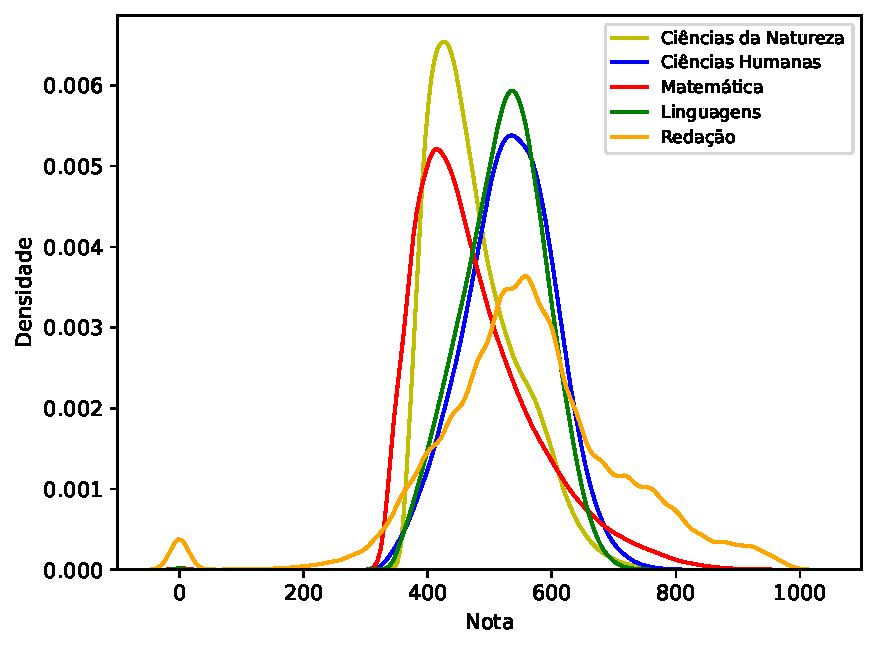
\includegraphics[width=\linewidth]{figuras/distribuicao_notas_feminino.pdf}
                    \caption{Feminino}
                \end{subfigure}
                \hfill
                \begin{subfigure}{\textwidth}
                    \centering
                    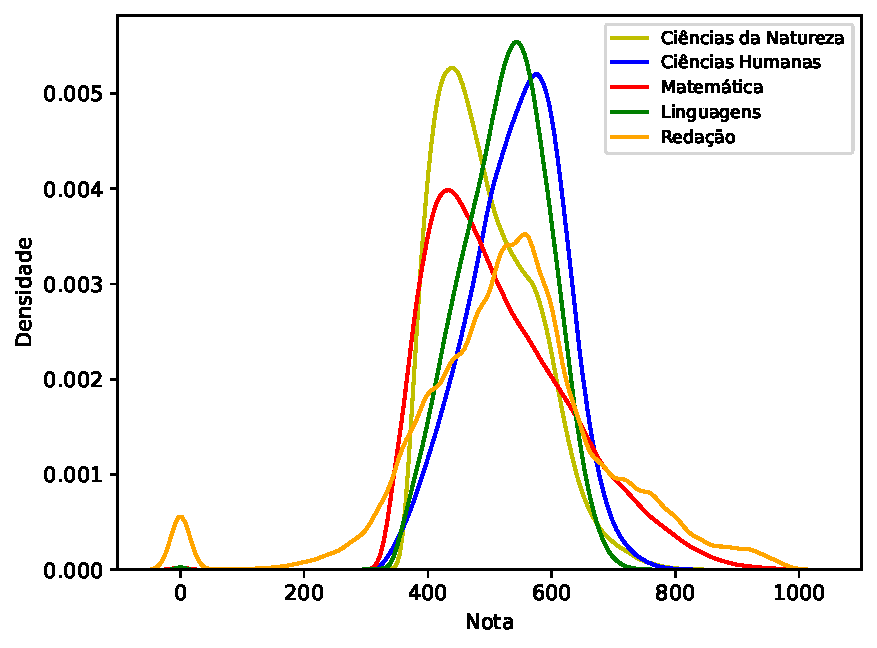
\includegraphics[width=\linewidth]{figuras/distribuicao_notas_masculino.pdf}
                    \caption{Masculino}
                \end{subfigure}
            
                \caption{Distribuição das notas do ENEM por gênero}
                \label{fig:nota-genero}
            \end{figure}
            
            \begin{figure}[h]
                \centering
            
                \begin{subfigure}{\textwidth}
                    \centering
                    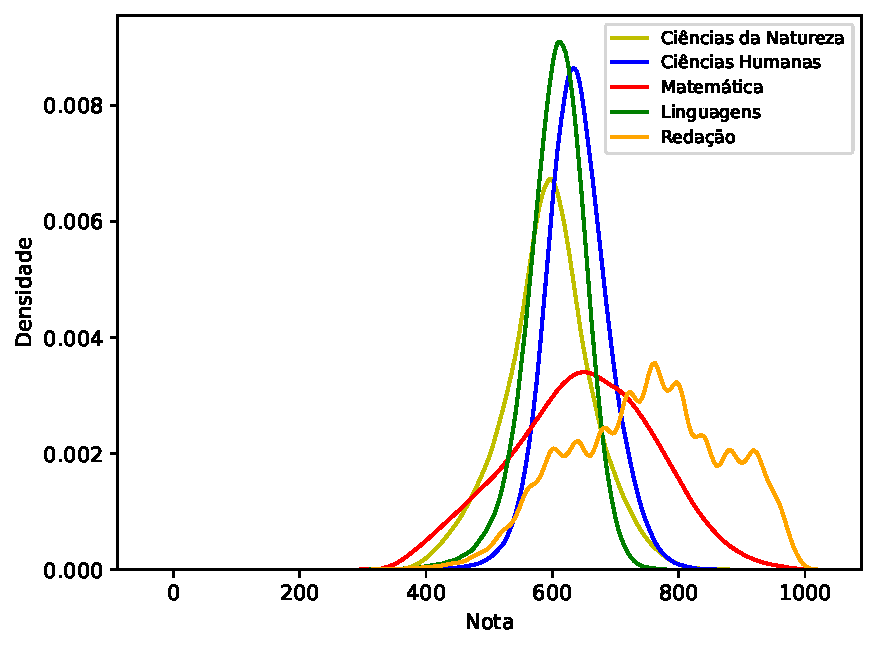
\includegraphics[width=\linewidth]{figuras/distribuicao_notas_aprovados.pdf}
                    \caption{Aprovado}
                \end{subfigure}
                \hfill
                \begin{subfigure}{\textwidth}
                    \centering
                    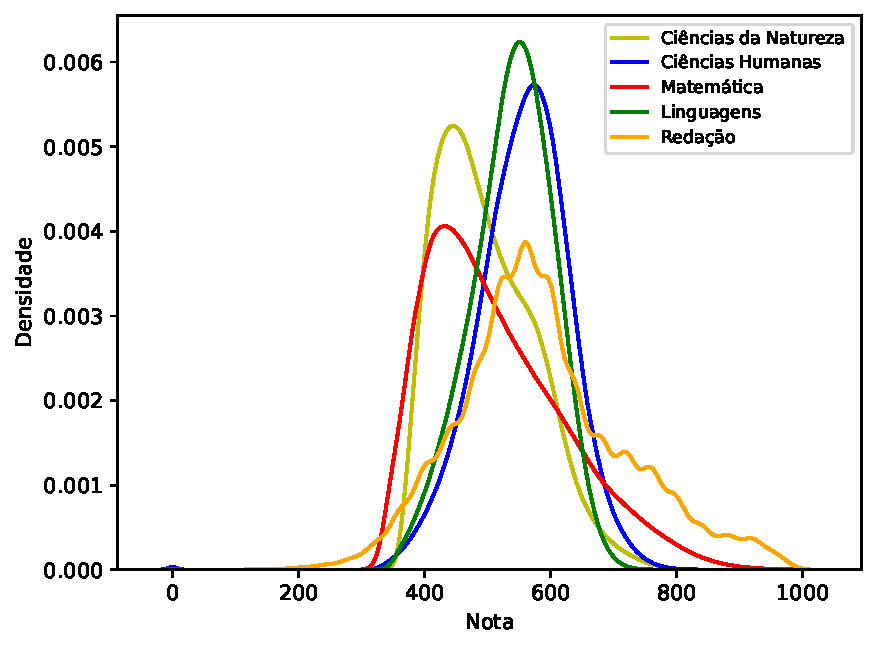
\includegraphics[width=\linewidth]{figuras/distribuicao_notas_nao_aprovados.pdf}
                    \caption{Não aprovado}
                \end{subfigure}
            
                \caption{Distribuição das notas do SISU por situação de aprovação}
                \label{fig:nota-aprovacao}
            \end{figure}
    
            \begin{table}[]
                \centering
                \begin{tabular}{ccc}
                \hline
                \textbf{Classificação}                        & \textbf{Feminino} & \textbf{Masculino} \\ \hline
                Educação                             & 6,29\%   & 1,81\%    \\ \hline
                Humanidades e artes                  & 8,94\%   & 7,69\%    \\ \hline
                Ciências sociais, negócios e direito & 22,24\%  & 20,85\%   \\ \hline
                Ciência                              & 13,01\%  & 21,85\%   \\ \hline
                Engenharia, manufatura e construção  & 9,76\%   & 19,96\%   \\ \hline
                Agricultura                          & 5,19\%   & 4,90\%    \\ \hline
                Saúde e bem-estar                    & 22,95\%  & 10,42\%   \\ \hline
                Serviços                             & 6,53\%   & 7,76\%    \\ \hline
                Não informado                        & 5,10\%   & 7,76\%    \\ \hline
                \end{tabular}
                \caption{Distribuição da classificação dos cursos do SISU por gênero}
                \label{tab:classificacao-curso-genero}
                \end{table}

                \begin{table}[]
                    \centering
                    \begin{tabular}{cc}
                    \hline
                    \textbf{Instituição de Ensino}                                   & \textbf{Porcentagem} \\ \hline
                    Universidade Federal do Maranhão                                 & 3,79\%               \\ \hline
                    Universidade Federal do Rio de Janeiro                           & 3,43\%               \\ \hline
                    Universidade Federal Fluminense                                  & 3,13\%               \\ \hline
                    Universidade Federal da Bahia                                    & 3,01\%               \\ \hline
                    Instituto Federal de Educação, Ciência e Tecnologia ds São Paulo & 2,63\%               \\ \hline
                    Universidade Federal do Piauí                                    & 2,60\%               \\ \hline
                    Universidade Federal da Paraíba                                  & 2,60\%               \\ \hline
                    Universidade Federal de Minas Gerais                             & 2,58\%               \\ \hline
                    Universidade Tecnológica Federal do Paraná                       & 2,29\%               \\ \hline
                    Universidade Federal de Pernambuco                               & 2,17\%               \\ \hline
                    \end{tabular}
                    \caption{Distribuição das 10 universidades com mais inscrições no SISU}
                    \label{tab:universidade-inscricao}
                    \end{table}

                    \begin{figure}[h]
                        \centering
                    
                        \begin{subfigure}{\textwidth}
                            \centering
                            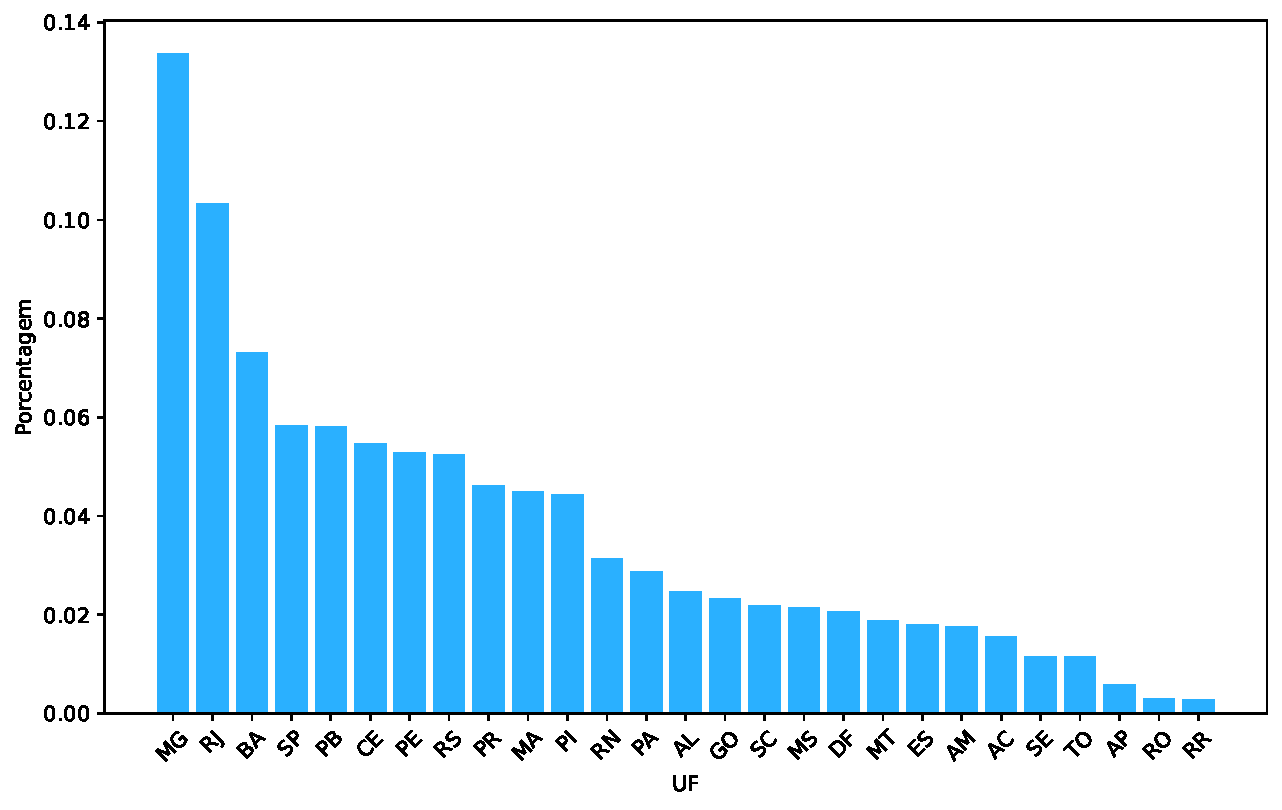
\includegraphics[width=\linewidth]{figuras/distribuicao_ies.pdf}
                            \caption{Inscrições em instituições de ensino}
                        \end{subfigure}
                        \hfill
                        \begin{subfigure}{\textwidth}
                            \centering
                            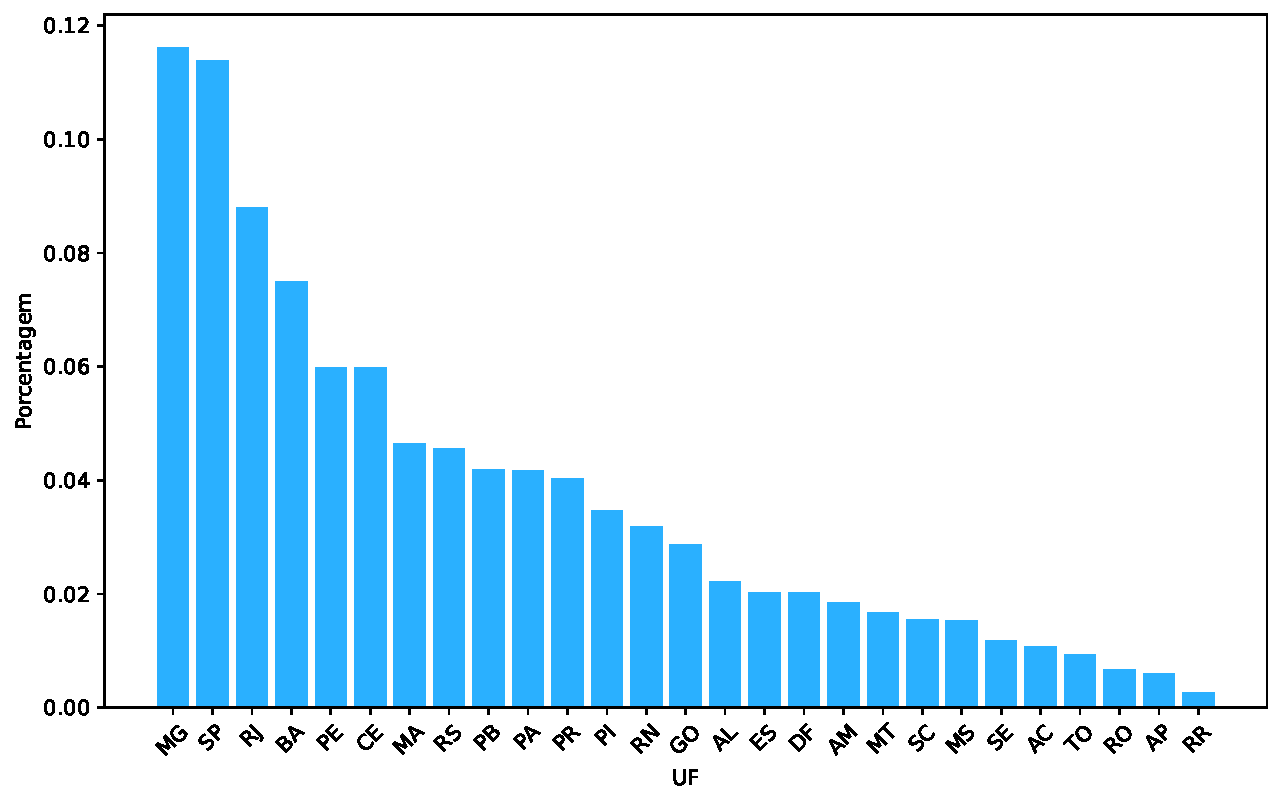
\includegraphics[width=\linewidth]{figuras/distribuicao_residencia_candidatos.pdf}
                            \caption{Residência dos candidatos}
                        \end{subfigure}
                    
                        \caption{Distribuição das unidades federativas no SISU}
                        \label{fig:distribuicao-uf}
                    \end{figure}